\begin{frame}{What are roll vortices ?}
 \begin{columns}
 \begin{column}{0.48\textwidth}
 \begin{itemize}
     \item  instabilities, scondary flows, coherent strcutures, ... = many names ! \\
     \item both from convection and shear flows
     \item "horizontally counter rotating vortices" across large horizontal regions
     \item sub mesoscale motion
\end{itemize}
 
 \end{column}
  \begin{column}{0.48\textwidth}
 \begin{figure}
     \centering
     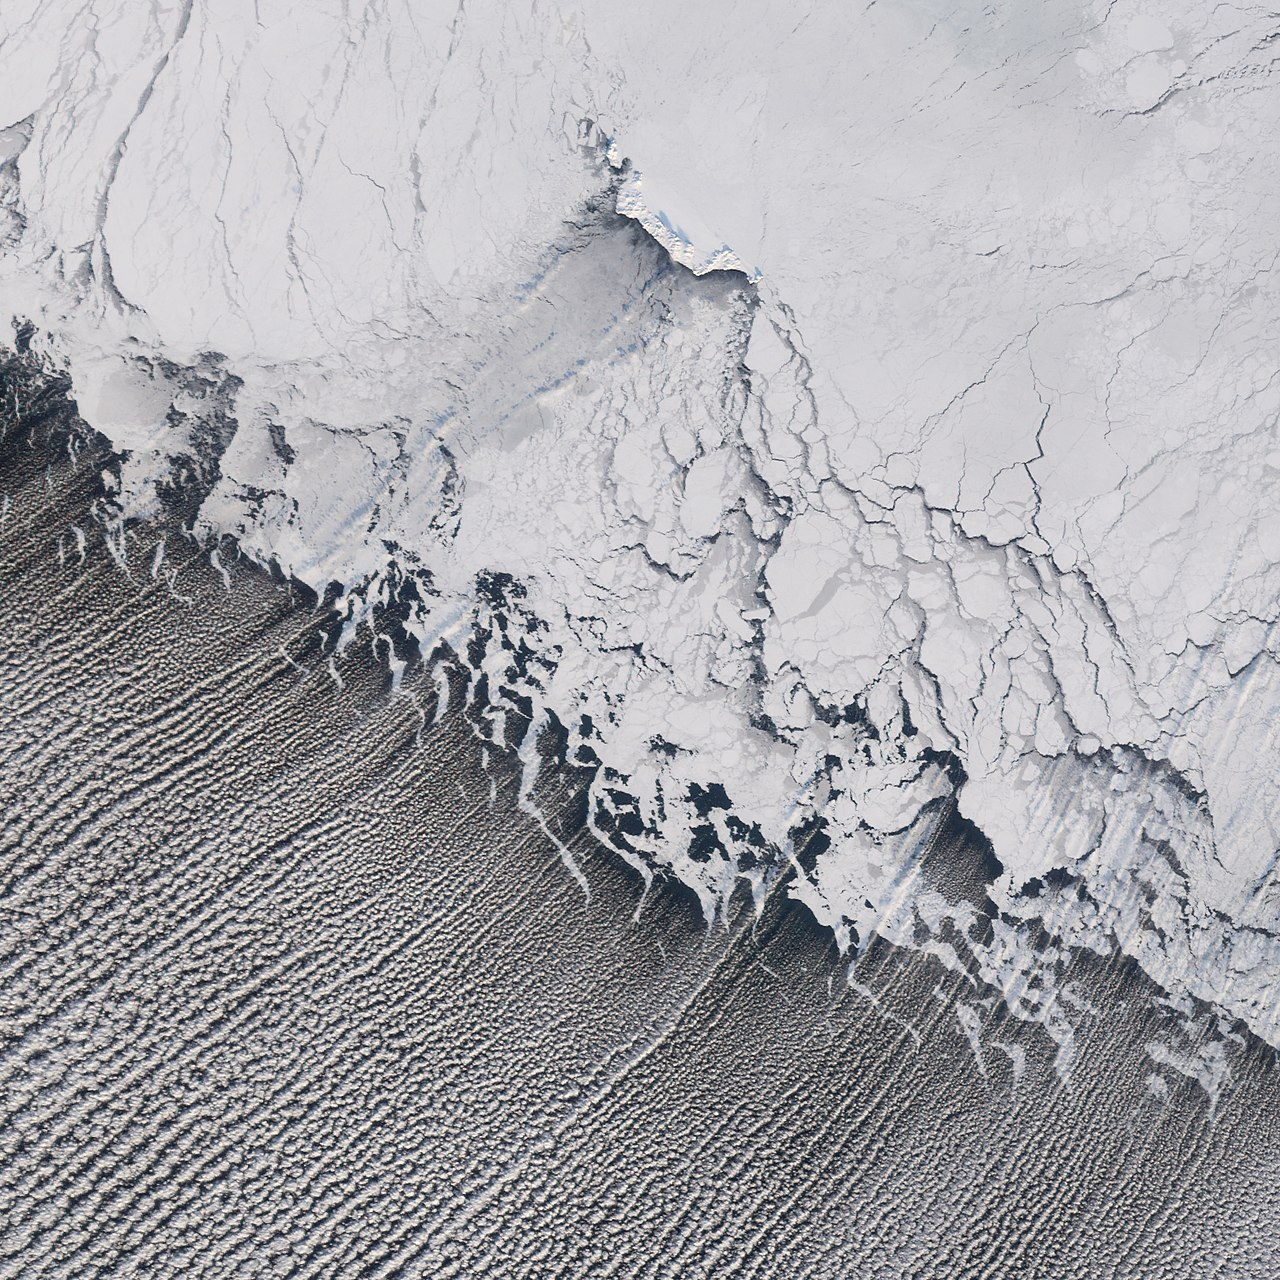
\includegraphics[width=1\linewidth]{FIGURES/roll.jpg}
     \caption{Horizontal rolls visualized by cloud streets over the Bering Sea (Wikipedia)}
     \label{fig:my_label}
 \end{figure}
 \end{column}
 \end{columns}

\end{frame}



\begin{frame}{Why interest in rolls ? }
\begin{itemize}
    \item Important role in \textbf{vertical transport} of momentum, heat, moisture and air pollutants in the CBL (\cite{etling_roll_1993})
    \item Important role in \textbf{interaction between surface and atmosphere} (\cite{liu_analytical_2009})
    \item Impact on the \textbf{ocean-air interaction} especially for strong winds (\cite{etling_roll_1993},  \cite{lfarh_impact_2024}) \\
    =\> Could be interesting to validate/improve existant air-sea flux parametrizations? 
    \item Could \textbf{initiate convection} (\cite{stensrud_wide_2022})
    \item 'little effort has been put forward by LES modellers' (in 1993) for having paramatrization of heat and momentum fluxes especially when large eddies (\cite{etling_roll_1993}) BUT some model the rolls explicitly in CBL parametrzation. (? to check \cite{brown_matching_1974})
\end{itemize}

\end{frame}

\begin{frame}{When do roll vortices happen ? }
From analytical experiment of a 2-layer atmosphere from (\cite{liu_analytical_2009}) + validated with numerical experiments (\cite{liu_numerical_2011}) the important conditions are 
\begin{itemize}
    \item presence of a \textbf{disturbing source}
    \item \textbf{instability} in the CBL
    \item \textbf{temperature jump} at the top of the CBL
    \item \textbf{stable layer} above the CBL: importance of stratified atm
    \item suitable \textbf{wind-shear} across the top of CBL
    \item appropriate \textbf{viscosity} in the CBL
\end{itemize}
main mechanism = interaction between gravity waves and convection... 
\end{frame}

\begin{frame}{Analytical model of roll vortices (\cite{liu_analytical_2009})}
Take linearized Boussinesq equation at the hydrostatic equilibrium of a steady-state perturbation, \textbf{with a Rayleigh friction term}. 
\begin{equation}
\label{eq:sys_NS}
\begin{cases}
(\underline V \cdot \underline \nabla )\underline u_h &= - \frac{1}{\rho_0} \underline \nabla_h p - \mu \underline u_h \\
(\underline V \cdot \underline \nabla)w &= - \frac{1}{\rho_0} \frac{\partial}{\partial z}p - \mu w \\
\underline \nabla \cdot \underline V &= 0 \\
(\underline V \cdot \underline  \nabla)b + wN^2 &= \frac{g}{c_p \overline T}q - \mu b
\end{cases}
\end{equation}
Find 'stable points' for $\dot X = F(X_0) = 0$. The stable points don't depend on $t$: it is a uniformly stable solution. 
\end{frame}

\begin{frame}{Questions on rolls}
\begin{itemize}
    \item relation with gravity waves ? 
    \item seems to be many research on rolls and sea breeze
\end{itemize}
\end{frame}

\begin{frame}{Simulation testROLLS: inputs}
But : tester pipeline + reproduire exp avec paramètres
\begin{columns}
 \begin{column}{0.38\textwidth}
    \begin{table}[H]
        \centering
        \begin{tabular}{c|c}
            $\Delta x$, $\Delta y$ (m) & 100 \\
            CSEA\_FLX & ECUME6  
        \end{tabular}
        \caption{Caption}
        \label{tab:my_label}
    \end{table}
 \end{column}
 \begin{column}{0.58\textwidth}
 \begin{figure}[T]
     \centering
     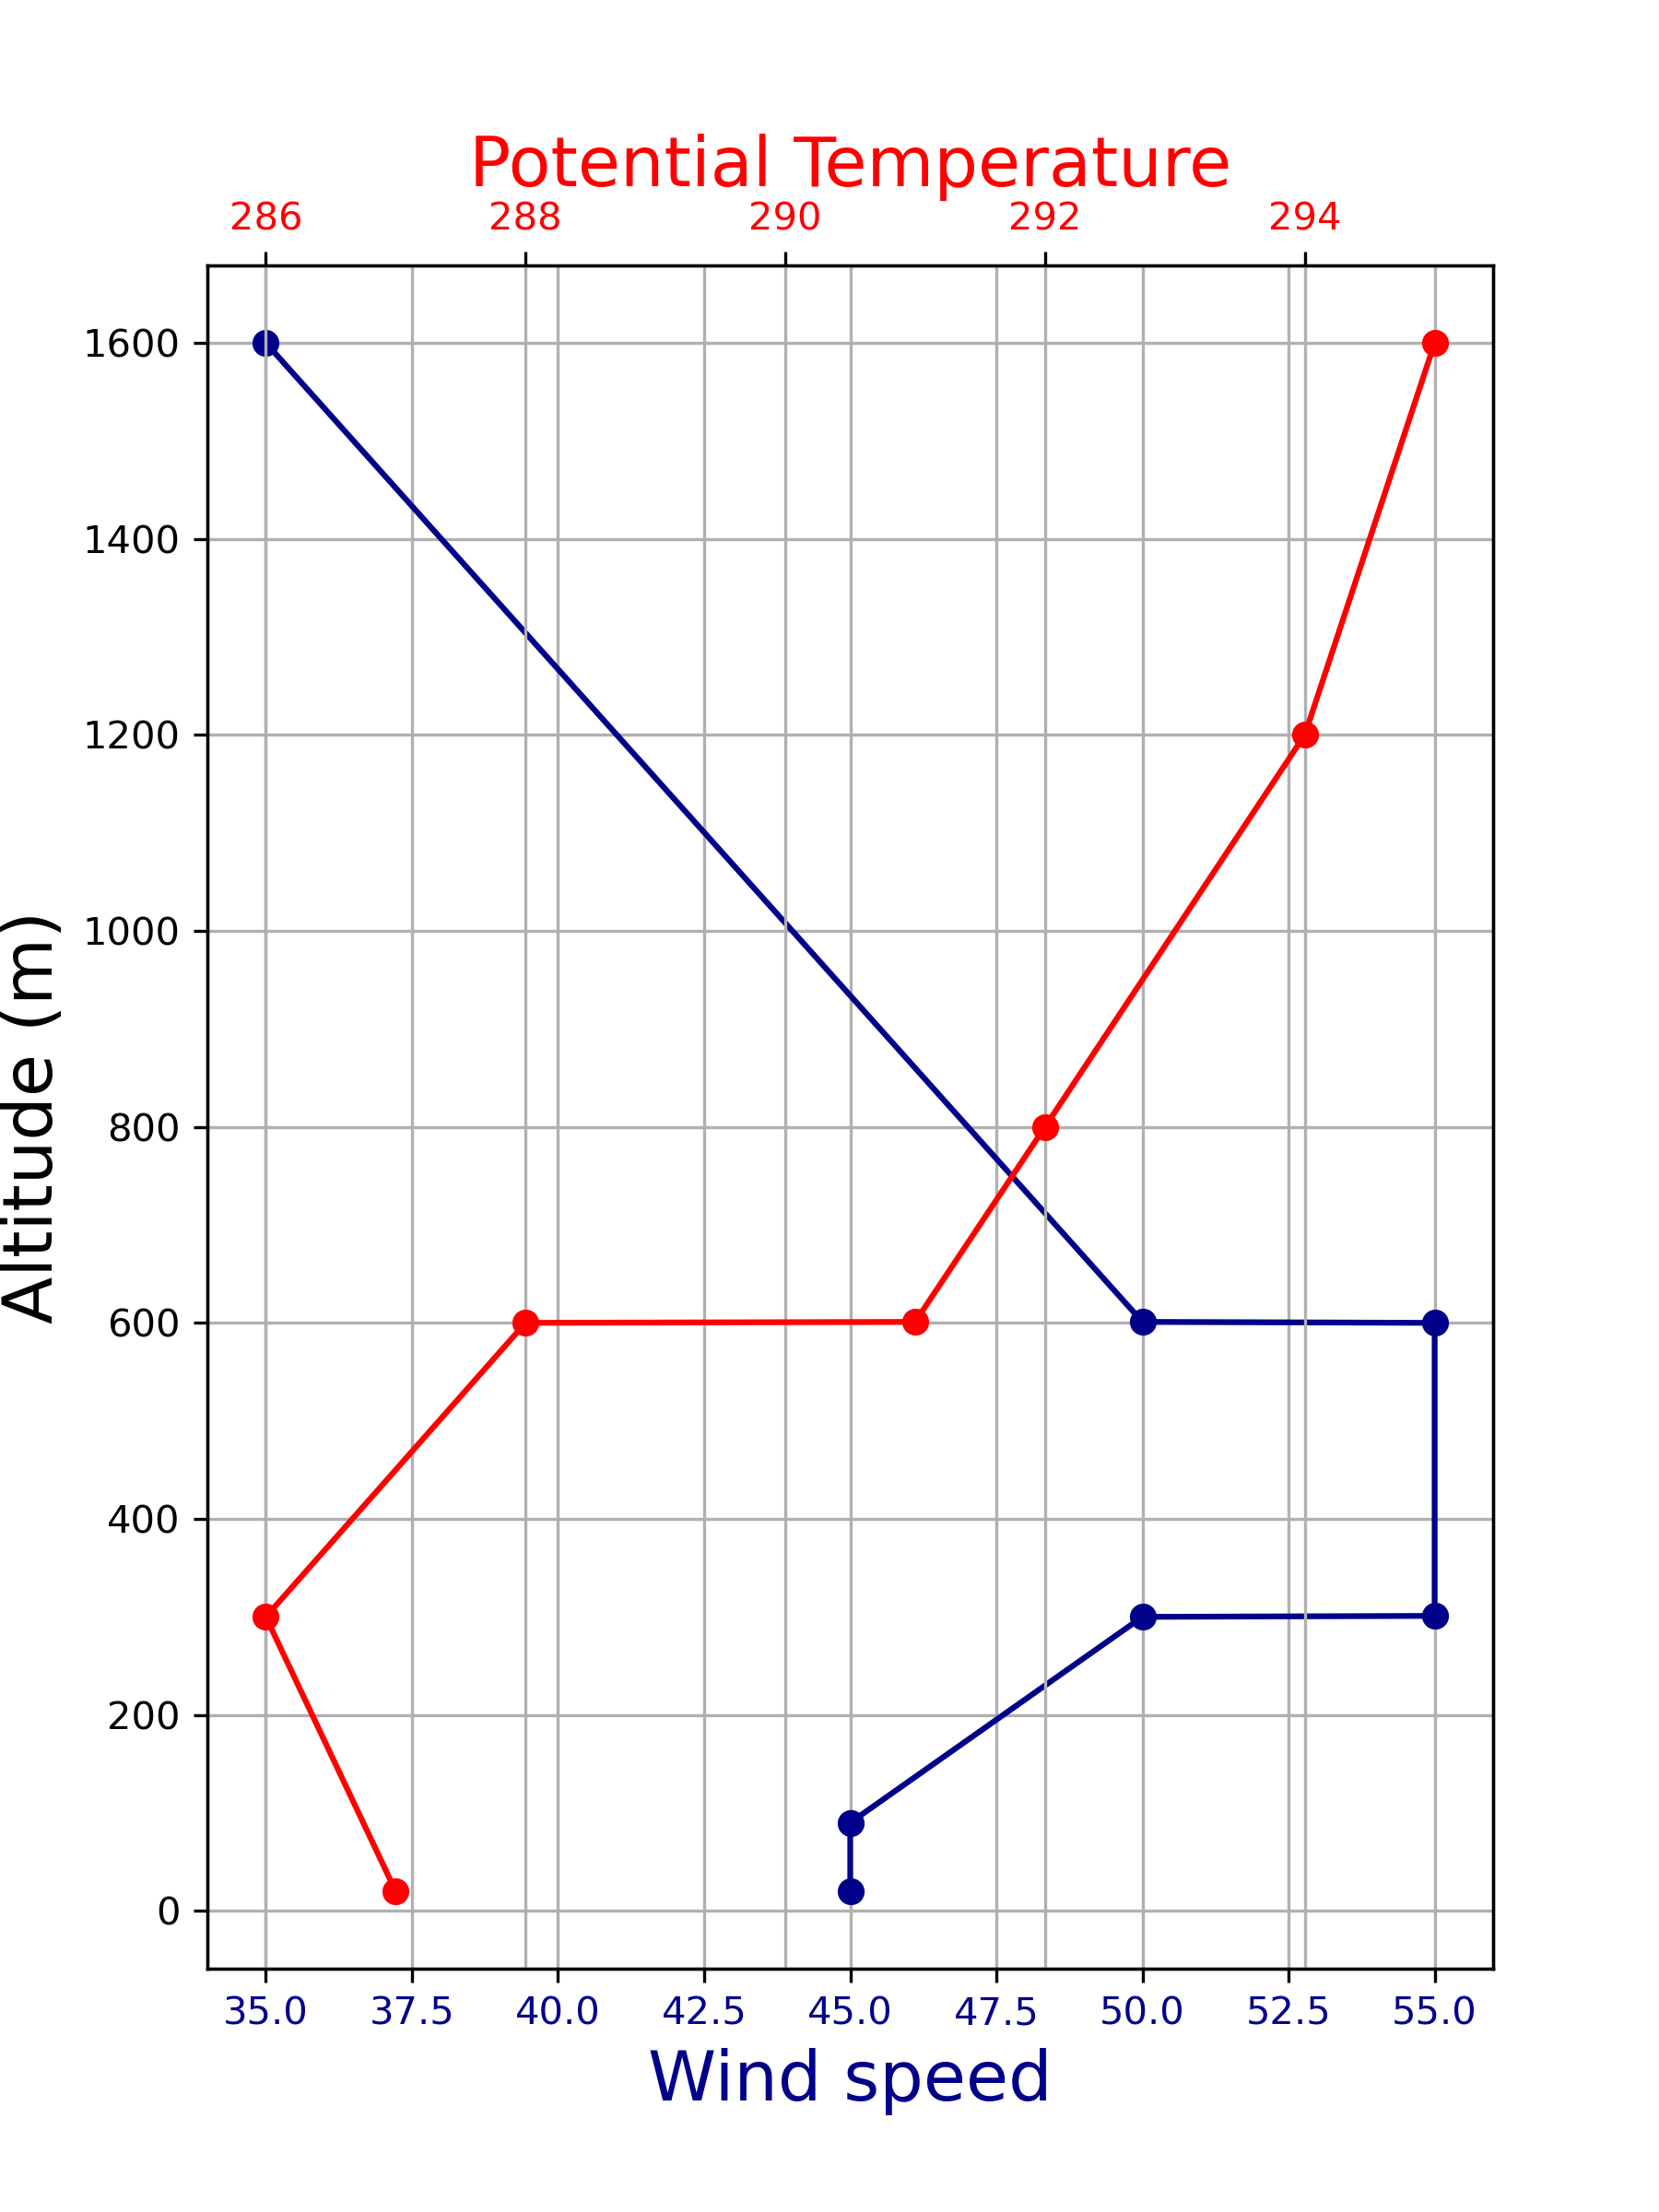
\includegraphics[width=0.45\textwidth]{FIGURES/param_in_testROLLS.png}
     \caption{Total wind and dry potential temperature profiles}
     \label{fig:my_label}
 \end{figure}
 \end{column}
 \end{columns}
\end{frame}

\begin{frame}{Simulation testROLLS: outputs}
     \begin{figure}[t]
     \centering
     
\includegraphics[width=0.85\textwidth]{FIGURES/wind_profiles.png}
     \caption{Wind profiles}
     \label{fig:my_label}
 \end{figure}
\end{frame}
\begin{frame}
     \begin{figure}[t]
     \centering
     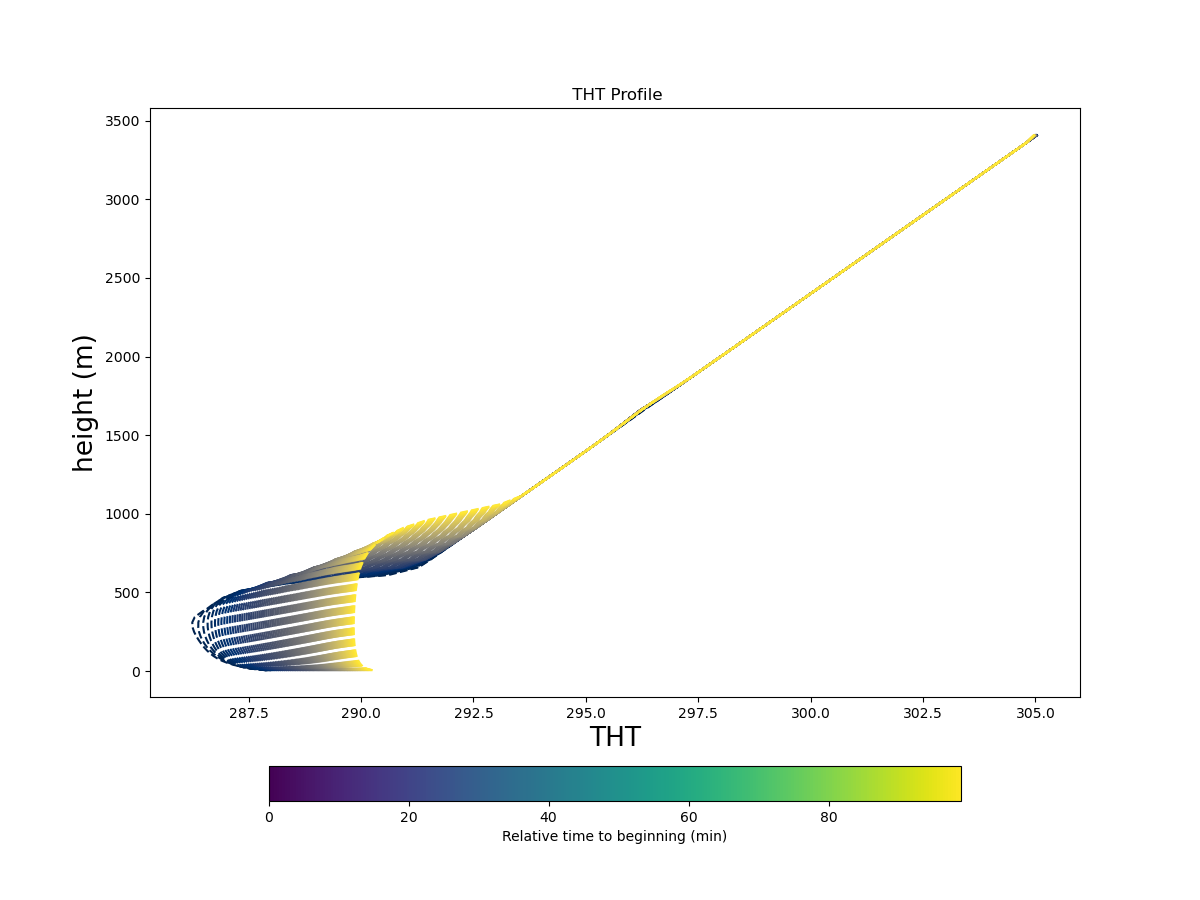
\includegraphics[width=0.85\textwidth]{FIGURES/temperature_profiles.png}
     \caption{temp profiles}
     \label{fig:my_label}
 \end{figure}
\end{frame}

\begin{frame}
     \begin{figure}[t]
     \centering
     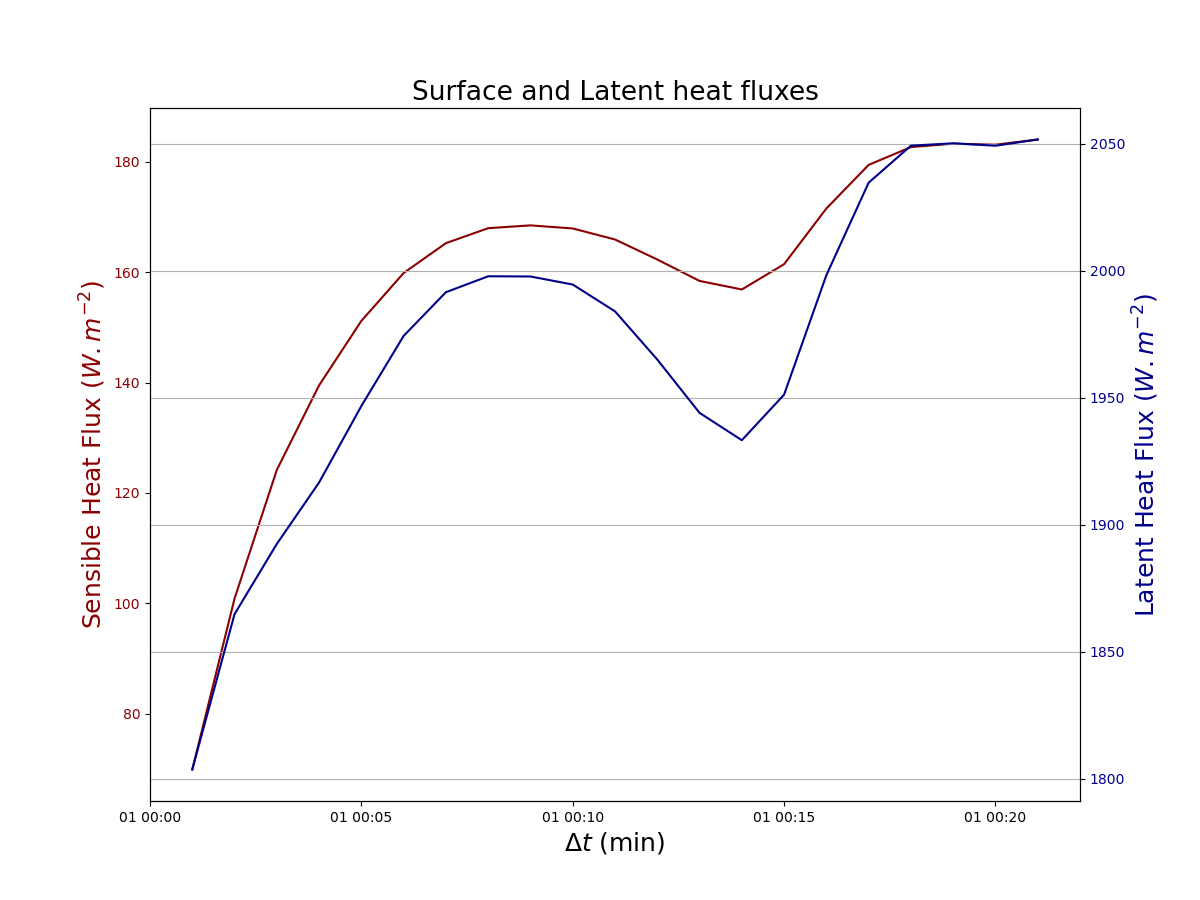
\includegraphics[width=0.85\textwidth]{FIGURES/fluxes.png}
     \caption{flux evolution}
     \label{fig:my_label}
 \end{figure}
    
\end{frame}

\begin{frame}{Lectures}
\begin{itemize}
    \item \cite{foster_2005}: importance ds formation cyclone trop. + 'étude préliminiaire' (?) pour paramtréisation. \textit{Downgradient param } pas possible car non-local, étude stabilité NL 
    \item \cite{wang_2023}: DL param of BL, difficultés à avoir des bonnes paramétrisation -$>$usage de DL pou maram toute la BL
    \item projet de lecture [\cite{swathi_unique_2025}] ?: rouleaux et moussons 
    \item projet de lecture [\cite{kepert_choosing_2012}] : choisir param pou BL des cyclones tropicaux
    \item projet lecture : lire sur Ekman BL et instabilites 
\end{itemize}
\end{frame}

